\documentclass {article}

\usepackage[utf8]{inputenc}
\usepackage{graphicx}
\usepackage{listings}
\usepackage{color}
\usepackage{float}

\definecolor{dkgreen}{rgb}{0,0.6,0}
\definecolor{gray}{rgb}{0.5,0.5,0.5}
\definecolor{mauve}{rgb}{0.58,0,0.82}

\lstset{frame=tb,
    language=C,
    aboveskip=3mm,
    belowskip=3mm,
    showstringspaces=false,
    columns=flexible,
    basicstyle={\small\ttfamily},
    numbers=left,
    numberstyle=\tiny\color{gray},
    keywordstyle=\color{blue},
    commentstyle=\color{dkgreen},
    stringstyle=\color{mauve},
    breaklines=true,
    breakatwhitespace=true,
    tabsize=3
}


\title{TP4 IA: Perceptron}
\author{ABDELMOUMENE Djahid}

\begin{document}
\maketitle

\section{Questions préliminaires}
Schéma de réseau:
\begin{figure}[H]
   \centering
   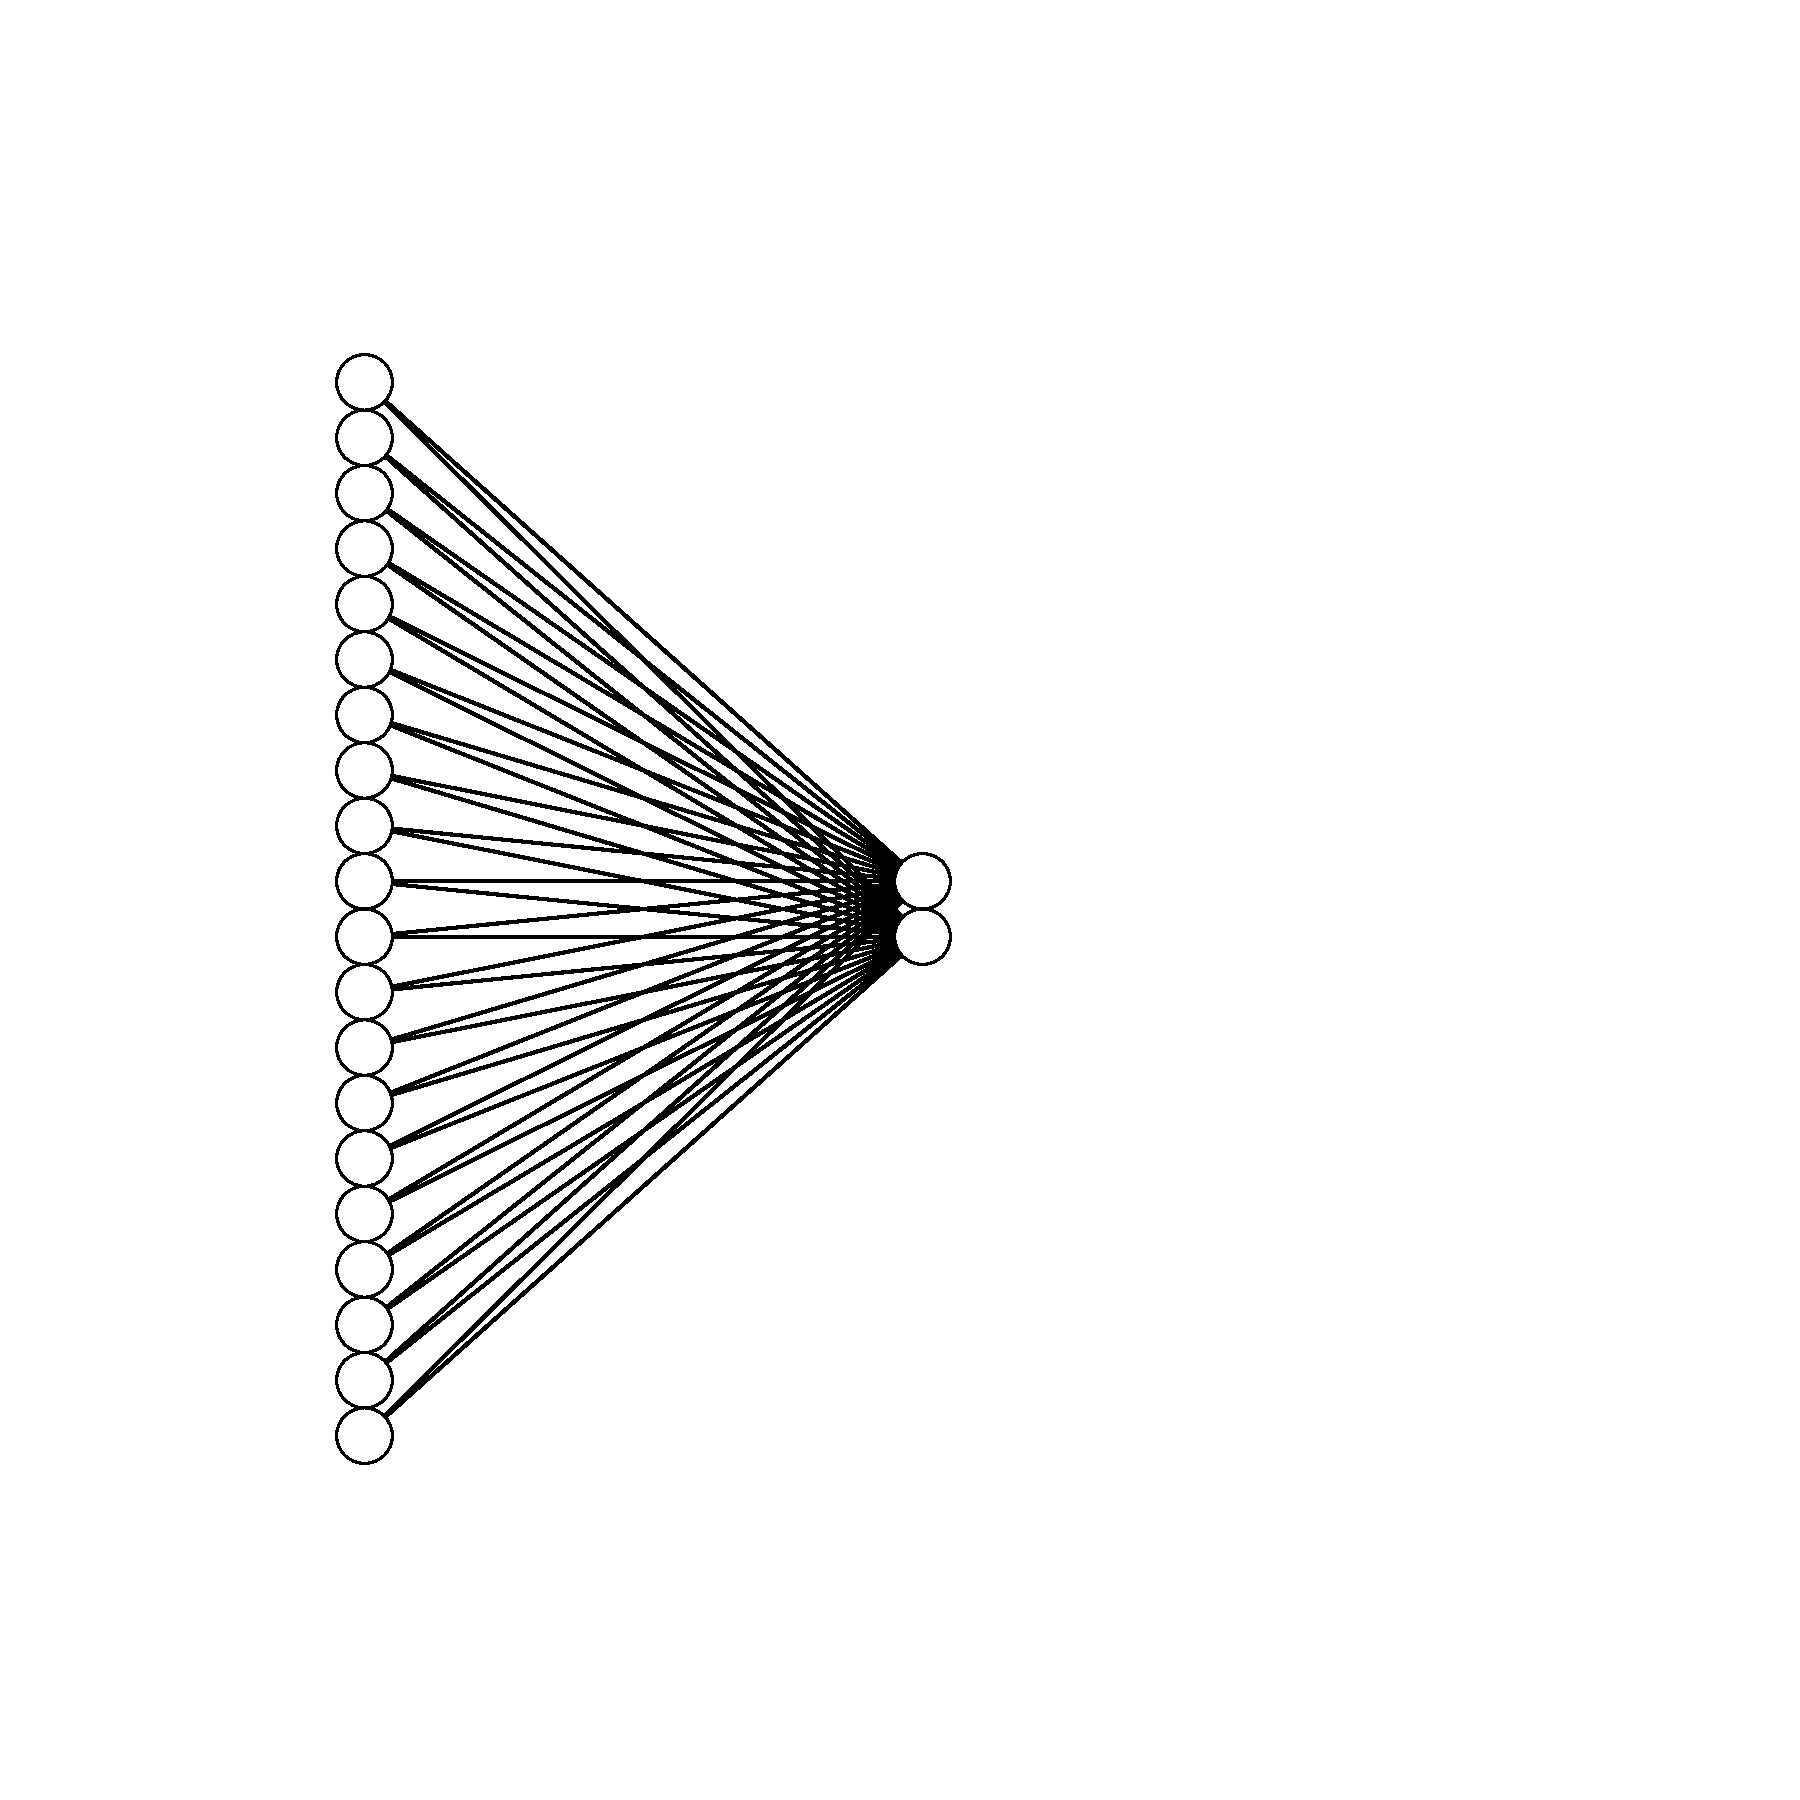
\includegraphics[height=20em]{ACnn.pdf}
   \caption{Schéma de réseau neurone pour classification de A et C}
\end{figure}

Structure de réseau de neurone:
\begin{lstlisting}
typedef struct neurone {
   float *weight;              // tableau de coefficients 
   float (*activation)(float); // la fonction d'activation
   float out;                  // la valeur de sortie
} NEURONE;

typedef struct network {
   int num_layers;   // le nombre de couches
   NEURONE **layers; // Les neurones d'entrees et de sortie
   float *biases;    // Un biais par couche
   int *sizes;       // les tailles de chaque couche
} NETWORK;
\end{lstlisting}

Les poids de réseau neurones sont initialisé avec des valeur aléatoires entre
0 et 1, les biais est mis à 0.\\

La propagation de neurone de sortie $j$ se fait par la formule suivant
\begin{equation}
   \sum^{input\_size}_{i=1} f(W_{i j} * e_{i} - \theta_{1})
\end{equation}

Pour l'apprentisage, on met les poids suivant ce formule:
\begin{equation}
   W_{ij}(t+1) = W_{ij} + \epsilon * (Sd^c(i) - Xout_{i}(i)) * Xin_{i}(t)
\end{equation}

Et pour le mise à jour de biais:
\begin{equation}
   \theta_{l}(t+1) = \theta_{l}(t) + \sum_{i=1}^{input\_size}\epsilon * Xin_{i}(t)
\end{equation}

L'apprentissage s'arrête lorsqu'on atteint un niveau d'erreur acceptable
prédefini.

\section{Question de compréhension}
L'apprentisage minimise une fonction d'erreur pour chaque neurone de sortie.\\

En cas de translation ou rotation de motif le réseau ne pourra pas s'adapter
parce que les données d'entrees sont limitées (2 motifs).

\begin{figure}[H]
   \centering
   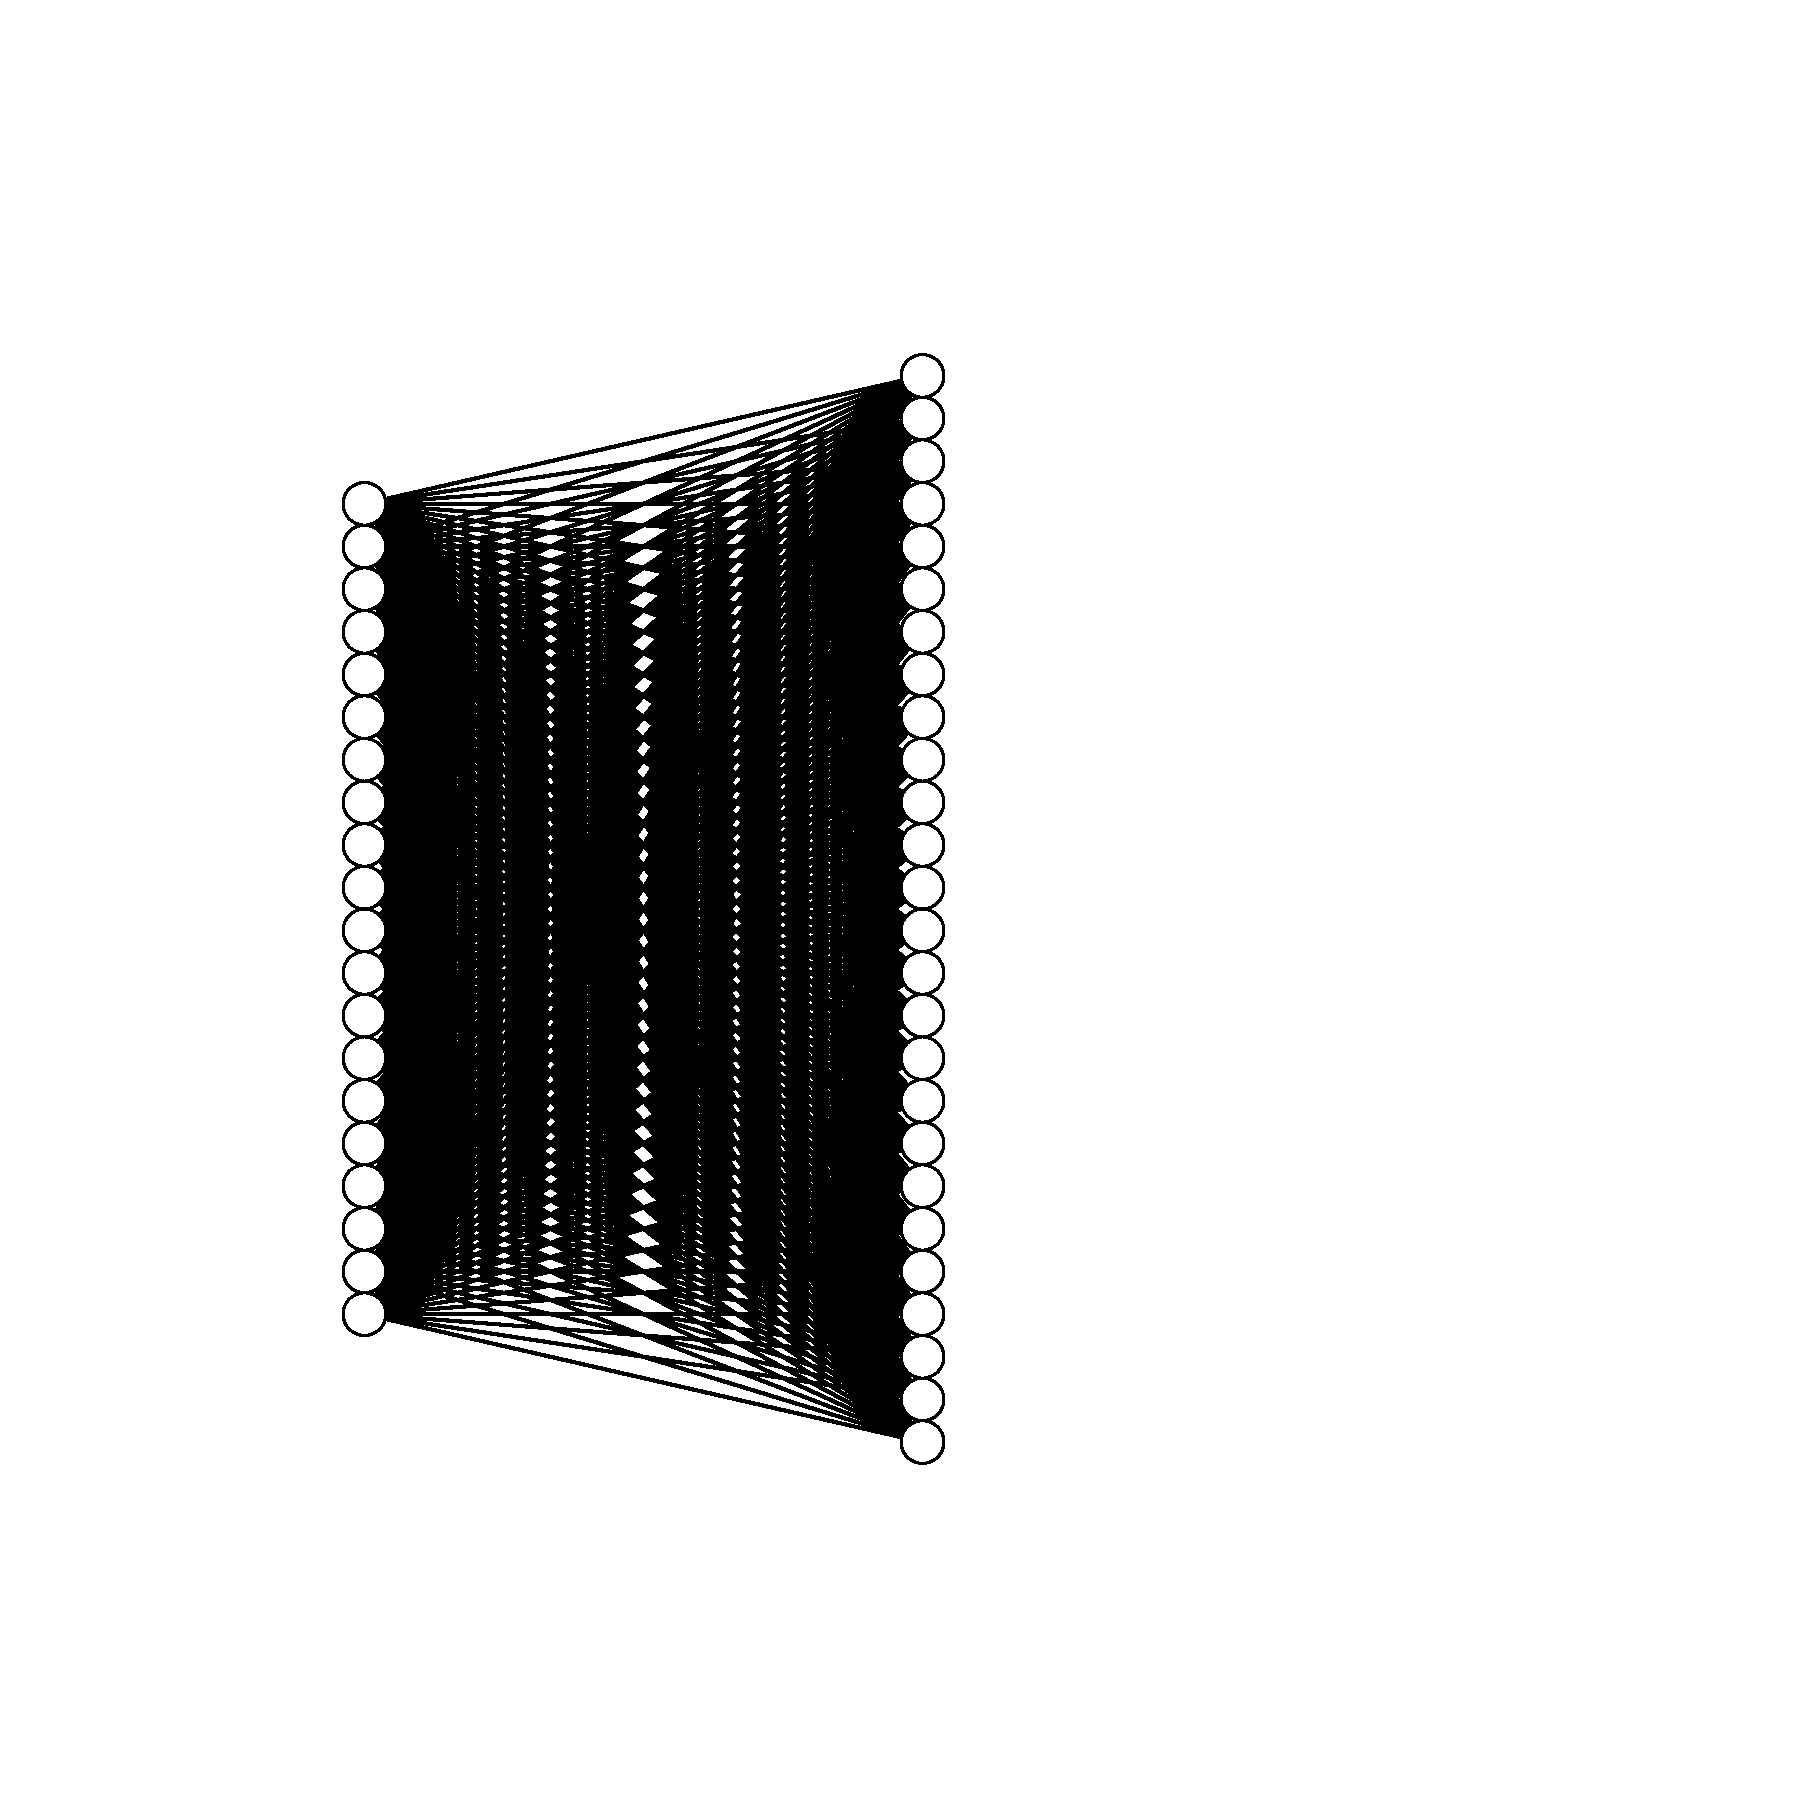
\includegraphics[height=20em]{AZnn.pdf}
   \caption{Schéma de réseau neurone pour classification de lettres}
\end{figure}



\end{document}
